\documentclass{standalone}
\usepackage{amsmath,amssymb,amsthm,stmaryrd}

\usepackage{tikz}
\usetikzlibrary{arrows,intersections}
\usetikzlibrary{fit,petri,topaths,calc}
\usetikzlibrary{shapes,decorations}
\usetikzlibrary{patterns}

\usepackage{adjustbox}
\usepackage{varwidth}

\usepackage{tikz}
\usetikzlibrary{fit}           
\usetikzlibrary{positioning}           
\usetikzlibrary{arrows,%shapes,snakes,automata,%
                petri,%
                topaths}%
\usetikzlibrary{calc}
\newcommand{\algo}[1]{\ensuremath{\mathsf{#1}}}

\begin{document}
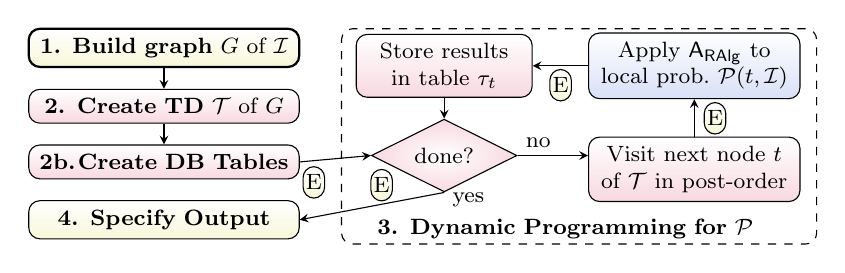
\begin{tikzpicture}[
	rounded corners,
	rect/.style={
		draw,
		rectangle,
		minimum height=4mm,
		top color=white,
		middle color=white,
	},
	dflatrect/.style={
		rect,
		bottom color=red!80!blue!15,
	},
	asprect/.style={
		rect,
		bottom color=blue!80!green!15,
	},
	decomprect/.style={
		rect,
		bottom color=yellow!80!black!15,
	},
	diam/.style={
		draw,
		diamond,
		shape aspect=2,
		sharp corners,
%		drop shadow,
		inner color=white,
		outer color=red!80!blue!15,
		%outer color=green!80!black!20,
	},
	font=\footnotesize,
	arrows=->,
	>=stealth,
]

%\matrix[column sep=4mm, row sep=4mm]{

\node [decomprect, thick, text width=32mm, text centered] (parse) {\textbf{1.\hspace{-0.02em} Build graph}~$G$ of~$\mathcal{I}$}; %&
\node [dflatrect, right=2em of parse, yshift=-.65em, text width=20mm, text centered] (populate) {Store results in table~$\tau_t$ }; %&
%
\node [decomprect,right=.1em of populate, xshift=0.5em, yshift=-.7em, inner sep=0.1em] (posttevent) {E};
%
\node [asprect, right=2em of populate, text width=24.5mm, text centered] (solve) {Apply $\algo{A_{RAlg}}$~to local prob.\ $\mathcal{P}(t,\mathcal{I})$}; %&
%
\node [decomprect,below=.1em of solve, xshift=0.75em, inner sep=0.1em] (pretevent) {E};
%\\
\node [dflatrect, below=.75em of parse, text width=32mm, text centered] (decompose) {\textbf{2. Create TD}~${\cal T}$ of~$G$}; %&
%
\node [dflatrect, below=.75em of decompose, text width=32mm, text centered] (createTables) {\textbf{2b. \hspace{-.35em}Create DB Tables}}; %&
\node [diam, below=0.75em of populate] (done) {done?};
\node [above right, xshift=1mm, yshift=1mm, inner sep=0] at (done.east) {no};
\node [below right, xshift=1mm, yshift=-0mm, inner sep=0] at (done.south) {yes};
%&
\node [dflatrect, below=1.35em of solve, text width=24.5mm, text centered] (traverse) {Visit next node~$t$ of~${\cal T}$ in post-order};
%\\

%& 
\node [decomprect, below=.75em of createTables, text width=32mm, text centered] (reconstruct)
{\textbf{4. Specify Output}};
%
\node [decomprect,right=-.2em of reconstruct,yshift=1.35em, xshift=0.3em, inner sep=0.1em] (preevent) {E};
%
\node [decomprect,right=2.25em of reconstruct,yshift=1.25em, xshift=0.3em, inner sep=0.1em] (postevent) {E};
%\\
%};
%
\node [xshift=15em,yshift=-3.2em,text width=58mm, text height=25mm,
draw, align=right,dashed] {\textbf{3. Dynamic Programming for~$\mathcal{P}$\qquad}\vspace{-2em}};

\draw (parse) -- (decompose);
\draw (decompose) -- (createTables);
\draw (createTables.east) -- (done.west);
\draw (done) -- (done-|traverse.west);
\draw (done.south) -- (reconstruct.east);
\draw (traverse) -- (solve);
\draw (solve) -- (populate);
\draw (populate) -- (done);
\end{tikzpicture}

\end{document}

%%% Local Variables:
%%% mode: latex
%%% TeX-master: t
%%% End:
